% !TEX root = main.tex
\section{Methods} % (fold)
\label{sec:methods}

\subsection{Producing the fragment PDB file}
The NMR structure of 4EBP2 used in this project is the same as in Bah \textit{et al.}
and has PDB ID \href{http://www.rcsb.org/pdb/explore/explore.do?structureId=2MX4}{\textcolor{blue}{2MX4}}.
Because 2MX4 includes 62 residues, we chose to simulate only a portion of the protein centered around one of the phosphorylated threonines, T37.
The full structure includes two known phosphothreonine sites, T37 and T46.
The fragment used in the simulations includes two residues before T37 and six after, comprising a nonamer with the sequence CTTPGTLF.
It extends to both ends of the loop in which T37 resides, as seen in Figure~\ref{fig:2MX4}.

\begin{figure}[h!]
  \caption{2MX4 in PyMOL. The fragment containing T37 used in the simulations is highlighted in green sticks.}
  \centering
    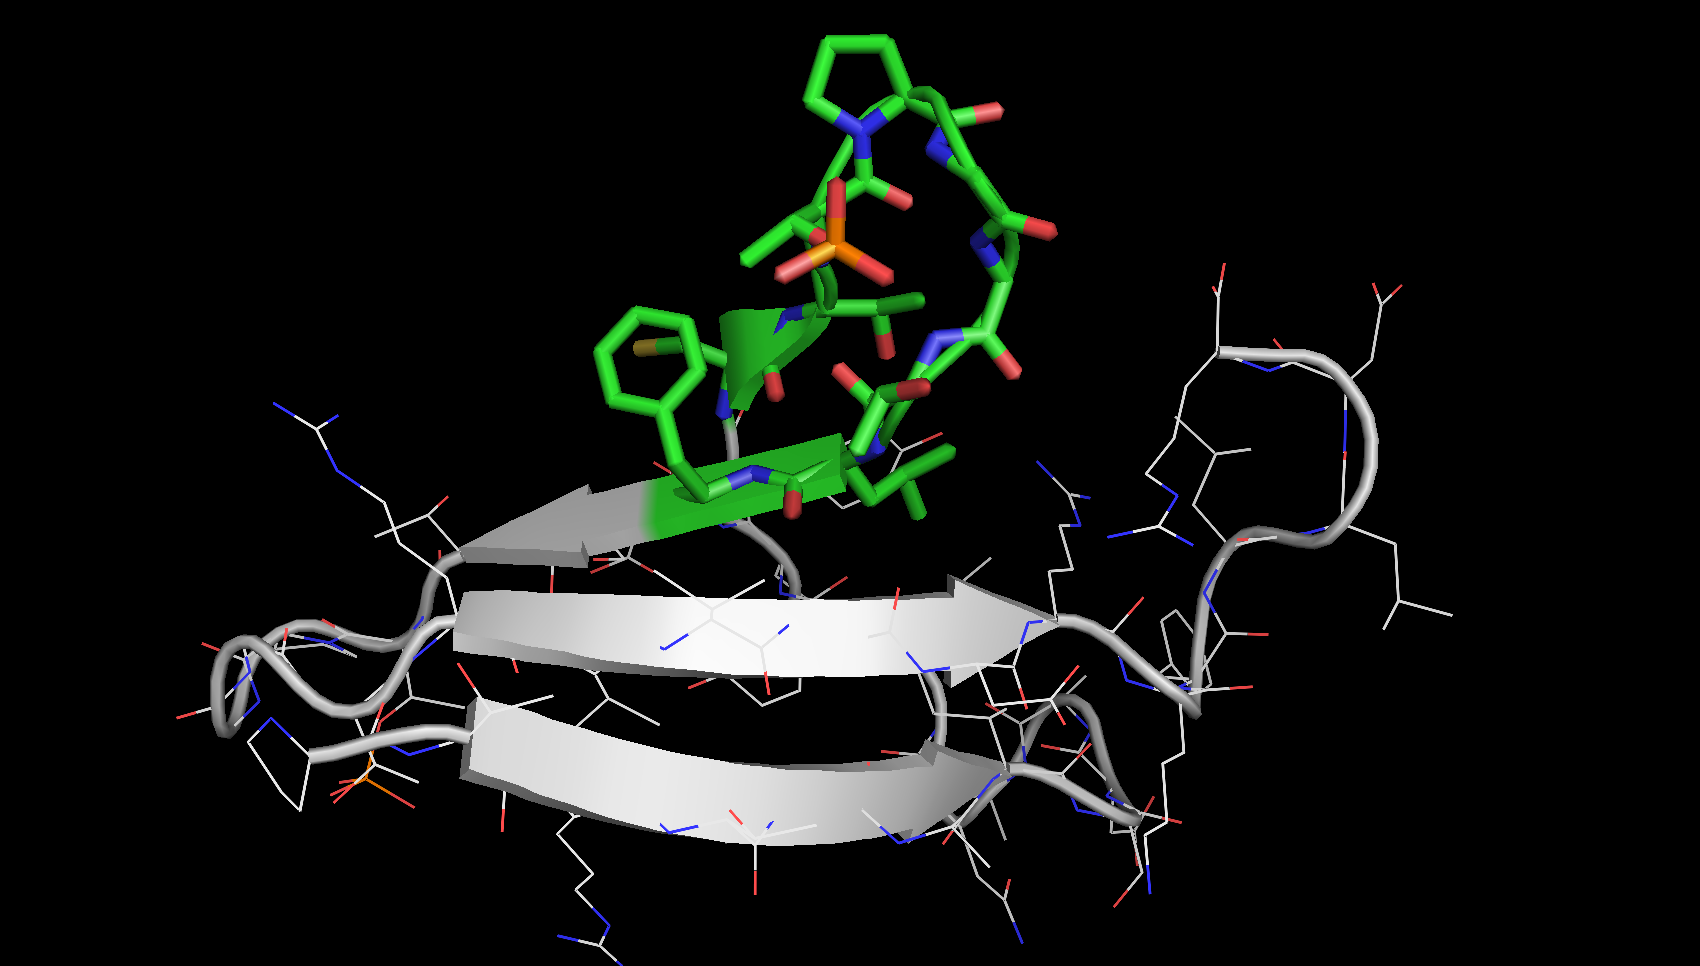
\includegraphics[width=0.5\textwidth]{2MX4}
  \label{fig:2MX4}
\end{figure}

\subsection{Capping the terminii}
Because the fragment does not have the same terminii as a native peptide, we capped the ends to mitigate unrealistic interactions.
For all versions of the fragment simulated, the N-terminus was acetylated and the C-terminus was methylamidated.
These caps were added with psfgen using the ACE and CT2 modifications on the N- and C-terminus, respectively.

\subsection{Dephosphorylating the fragment}
Talk about how we created unphosphorylated peptides.

Talk about how we created extended phosphorylated and unphosphorylated peptides.

Talk about how we created the PSF file.

Talk about the simulations we submitted. Talk about the automation scripts we wrote.

% section methods (end)
